\section{Research via artifacts}
Our research methodology applied and extended the growing knowledge of mining
software repositories~\cite{msr08}. Figure~\ref{fig:Framework} illustrates the
process of mining and leveraging software artifacts for research as we
conceptualize it. The goal is to study different kinds of \emph{Software
Development Activities}, such as planning, designing, implementing, or testing a
product. With the use of \emph{integrated development environments}, the
activities are recorded. In highly integrated collaboration development
environments such as Jazz, the record of development activities are kept in the
form of different artifacts such as plans, work items, or source code changes. We
opted to infer knowledge from the created artifacts, because gathering data
directly from the developers, through surveys or interviews, are often highly
invasive and very time consuming for researchers.


 \begin{figure}[t]
	\begin{center}
	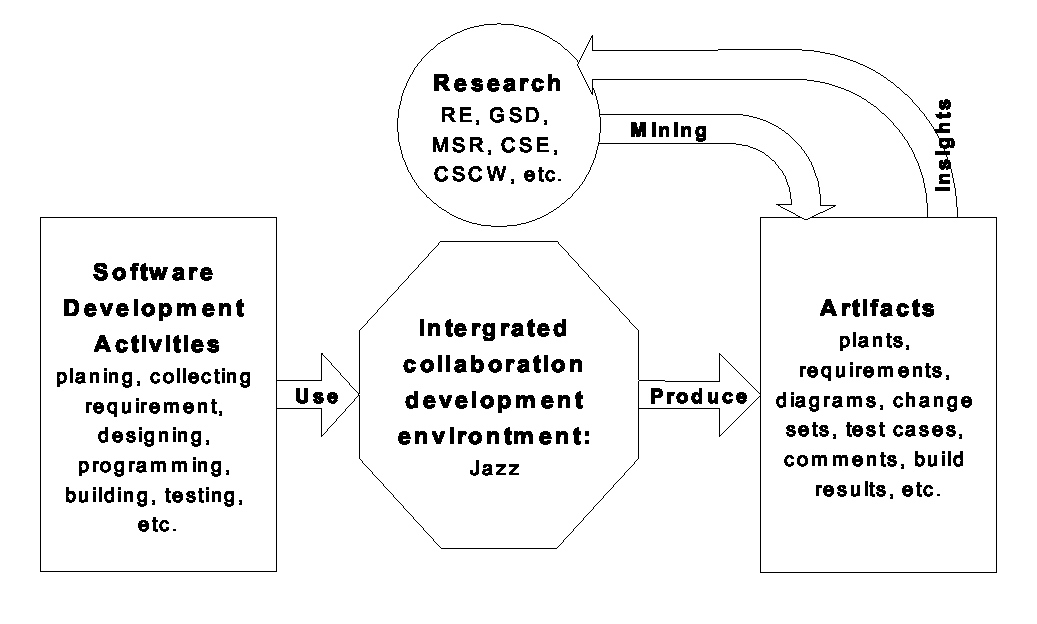
\includegraphics[width=.99\columnwidth]{./Figures/Figure01Framework}
	\caption{The research via artifacts process}
	\label{fig:Framework}
	\end{center}
\end{figure}

The mining and studying of development artiacts has its own specific
challenges as well. Two main challenges are:
\begin{enumerate}
\item The complexity of the data mining task.
\item The validity of insights obtained through the artifacts.
\end{enumerate}
The first challenge is a technical one. It raise questions such as ''How to
get access to the data?''. The data mining process can be very complex and
sometimes impossible. As we will explain in sbsequent sections, it requires
careful planing and implementation. The second challenge is on the research level. By
doing research via artifacts, we have to make inferences about the software
development activities through the artifacts it produces. This makes it hard to
interpret the result. The main questions center around ''How to interpret the
artifacts?'' and ''Is our interpretation valid?''.

The importance of these challenges depends on the point of view. For the
development team the first challenge is more relevant because extracting data
from a repository might crash it or delay the development process in other ways.
Whereas the second challenge is of more relevance to research. Researchers are
always interested in new findings, growing, or validating the body of knowledge.
After leveraging the two point of views, the big question that we are trying to
answer is: How to build a Jazz data mining tool that minimizes the effort of
both the development team and the researchers, and maximizes the validity of our
study? Before we discuss our approach to addressing this question, we briefly
describe the IBM Jazz project in the next section and explain why we
decided to build the data mining tool.
